\documentclass{template/openetcs_article}
% Use the option "nocc" if the document is not licensed under Creative Commons
%\documentclass[nocc]{template/openetcs_article} 
\usepackage[pdftex]{hyperref}
\usepackage{lipsum,url}
\usepackage{xspace}
\usepackage{graphicx}
\usepackage{fixme}
\usepackage{lscape} 
\usepackage{pgfgantt}
\usepackage{adjustbox}
\usepackage{datetime}
\usepackage{listings}
\usepackage{placeins}

\usepackage{float}
\floatstyle{plain}
\newfloat{listing}{thp}{lop1}[section]
\floatname{listing}{Listing}



%user specified macros


\newcommand{\VV}{Verification \& Validation\xspace}
\newcommand{\vv}{verification \& validation\xspace}

\def\CC{{C\nolinebreak[4]\hspace{-.05em}\raisebox{.4ex}{\tiny\bf ++}}}

\newcommand{\bitwalker}{\mbox{\texttt{Bitwalker}}\xspace}

\newcommand{\poke}{\mbox{\texttt{Bitwalker\_Poke}}\xspace}
\newcommand{\peek}{\mbox{\texttt{Bitwalker\_Peek}}\xspace}
\newcommand{\acsl}{\mbox{\textsf{ACSL}}\xspace}
\newcommand{\isoc}{\mbox{\textsf{C}}\xspace}
\newcommand{\framac}{\mbox{\textsf{Frama-C}}\xspace}
\newcommand{\framacwp}{\mbox{\textsf{Frama-C\slash WP}}\xspace}
\newcommand{\why}{\mbox{\textsf{Why}}\xspace}
\newcommand{\wpframac}{\mbox{\textsf{WP}}\xspace}
\newcommand{\altergo}{\mbox{\textsf{Alt-Ergo}}\xspace}
\newcommand{\qed}{\mbox{\textsf{Qed}}\xspace}
\newcommand{\cvc}{\mbox{\textsf{CVC4}}\xspace}
\newcommand{\z}{\mbox{\textsf{Z3}}\xspace}
\newcommand{\coq}{\mbox{\textsf{Coq}}\xspace}
\newcommand{\cealist}{\mbox{\textsf{CEA LIST}}\xspace}

\newcommand{\inl}[1]{\lstinline[style=inline]{#1}}


%Defining C-Code Environment

\usepackage{courier} 
\usepackage{listings}
\usepackage{color} 

% fix bug with listing under texlive-2014
% see https://lists.debian.org/debian-tex-maint/2014/06/msg00209.html

\makeatletter
\renewcommand\lstinline[1][]{%
  \leavevmode\bgroup % \hbox\bgroup --> \bgroup
  \def\lst@boxpos{b}%
  \lsthk@PreSet\lstset{flexiblecolumns,#1}%
  \lsthk@TextStyle
  \ifnum\iffalse{\fi`}=\z@\fi
  \@ifnextchar\bgroup{%
  \ifnum`{=\z@}\fi%
  \afterassignment\lst@InlineG \let\@let@token}{%
  \ifnum`{=\z@}\fi\lstinline@}}
\makeatother


%\definecolor{darkred}		{rgb}{0.60,0.00,0.00}
\definecolor{coACSLBehavior}	{rgb}{0.30,0.00,0.00}
\definecolor{coASCL}		{rgb}{0.00,0.10,0.00}
\definecolor{coASCLKeyword}	{rgb}{0.00,0.10,0.10}
\definecolor{darkgreen}		{rgb}{0.00,0.40,0.00}
%\definecolor{red}		{rgb}{0.98,0.00,0.00}
\definecolor{darkblue}		{rgb}{0.00,0.00,0.60}
%\definecolor{lightblue}		{rgb}{0.60,0.80,1.00}
%\definecolor{lightred}		{rgb}{1.00,0.60,0.60}
\definecolor{coCKeyword}	{rgb}{0.00,0.00,0.60}

\lstdefinestyle{acsl-block}
{	emph=[1]{assert, assumes, assigns, axiom, axiomatic, decreases, ensures,
                 ghost, invariant, lemma, logic, loop, predicate,
		 reads, requires, variant},
	emphstyle=[1]{\bfseries\color{coASCLKeyword}},
	emph=[2]{behavior, behaviors, complete, disjoint, for:},
	emphstyle=[2]{\bfseries\color{coACSLBehavior}},
	emph=[3]{typedef, int, char, integer, real, bool, size_type, value_type, uint8_t,  uint64_t},
	emphstyle=[3]{\bfseries\color{coCKeyword}},
	escapeinside={//`}{`//},
	morecomment=*[l][\color{coASCL}]{//@},
	morecomment=*[s][\color{coASCL}]{/*@}{*/},
	moredelim=*[is][\bfseries]{|*}{*|},
	%emphstyle=[3]{\ttfamily}
	}

\lstdefinestyle{func-decl}
{	emph=[1]{assert, assumes, assigns, axiom, axiomatic, decreases, ensures,
                 ghost, invariant, lemma, logic, loop, predicate,
		 reads, requires, variant},
	emphstyle=[1]{\bfseries\color{coASCLKeyword}},
	emph=[2]{behavior, behaviors, complete, disjoint, for:},
	emphstyle=[2]{\bfseries\color{coACSLBehavior}},
	emph=[3]{integer, real, size_type, value_type},
	emphstyle=[3]{\bfseries\color{coCKeyword}},
	escapeinside={//`}{`//},
	morecomment=*[l][\color{coASCL}]{//@},
	morecomment=*[s][\color{coASCL}]{/*@}{*/},
	moredelim=*[is][\bfseries]{|*}{*|},
    frame=none,
    numbers=none
	%emphstyle=[3]{\ttfamily}
	}

\lstdefinestyle{acsl-inline}
{	emph=[1]{assert,assigns, assumes, axiom, axiomatic, decreases, ensures, ghost, invariant, lemma, logic, loop,
             predicate, reads, requires, return, variant },
	emphstyle=[1]{\bfseries\color{coASCLKeyword}},
	emph=[2]{behavior, behaviors, complete, disjoint, for:},
	emphstyle=[2]{\bfseries\color{coACSLBehavior}},
	emph=[3]{typedef, int, char, integer, real, bool, size_type, value_type, uint8_t,  uint64_t},
	emphstyle=[3]{\bfseries\color{coCKeyword}},
	morecomment=*[l][\color{coASCL}]{//@},
	morecomment=*[s][\color{coASCL}]{/*@}{*/},
	moredelim=*[is][\bfseries]{|*}{*|}
}

\lstdefinestyle{inline}
{      % basicstyle = \ttfamily\small\color{coASCL},
	keywordstyle = \ttfamily\small\color{coASCL},
	stringstyle=\color{coASCL},
	style=acsl-inline,
	breaklines= false
}

\lstset{%
  language=C++,
  defaultdialect=ansi,
  basicstyle=\small\ttfamily,
  commentstyle=\small\color{darkgreen},
  keywordstyle=\small\bfseries\color{darkblue},
  stringstyle=\small\color{darkgreen},
  tabsize = 2,
  showspaces=false,
  showtabs=false,
  columns=fixed,  
  frame=none,  
  breaklines=true,
  showstringspaces=false,
  xleftmargin=0.2cm,
  %rangeprefix=//label, % to specify a certain range from a file
  %rangesuffix=;, % to be shown
  %includerangemarker=false,
	numbers=none
}


\graphicspath{{./template/}{.}{./images/}}
\begin{document}
\frontmatter
\project{openETCS}

%Please do not change anything above this line
%============================
% The document metadata is defined below

%assign a report number here
\reportnum{OETCS/WP4/D4.2.2}

%define your workpackage here
\wp{Work Package 4: ``Validation \& Verification Strategy''}

%set a title here
\title{First Validation and Verification Report on Implementation/Code}

%set a subtitle here
%\subtitle{Description of Work}

%set the date of the report here
\date{November 2013}

%define a list of authors and their affiliation here

\author{Marc Behrens}

\affiliation{WP4 Leader}
 
\author{Jens Gerlach}

\affiliation{WP4.3 Task Leader (Validation and Verification of Implementation/Code)}

% define the coverart
\coverart[width=350pt]{openETCS_EUPL}

%define the type of report
\reporttype{Description of work}



\begin{abstract}
%define an abstract here

  This work package will comprise the activities concerned with
  verification and validation within openETCS. This includes \vv of
  development artifacts, that is, showing that models and code
  produced correctly express or implement what they are supposed
  to. And also, methods and tools to perform such tasks will be
  evaluated with the goal of assembling a suitable method and tool
  chain to support a full development.

\end{abstract}

%=============================
%Do not change the next three lines
\maketitle
\tableofcontents
\listoffiguresandtables
\newpage
%=============================

% The actual document starts below this line
%=============================


%Start here

\section{Introduction}


\section{Formal Verification of Bitwalker}
\label{sec:fokus}


In this section we describe our work on the formal verification
of the so-called Bitwalker.
The Bitwalker shall read bit sequences from a bit stream 
and convert them to an integer. Furthermore, it shall
convert an integer into a bit sequence and write it into a bit stream.
Therefore, the Bitwalker has a read and a write function, namely \peek and \poke.

Our aim is to verify the functionality of
\peek and \poke
as well as their correct interaction.
Furthermore, we want to verify some robustness cases for \peek and \poke
and the absence of run time errors for both functions.
We won't take into account any complexity requirements.

We introduce a method to achieve these goals in section~\ref{plan}.
Moreover, it is our intention
to elaborate the method and in particular the associated tools.

Subsequently, we use the method for \peek and \poke
in section~\ref{peek} and~\ref{poke}, respectively.
We provide an informal specification, an implementation and
a formal specification for each function and
present what could have been verified for the implementation.

We discuss the interaction of these functions in section~\ref{interaction}
where we show how the interaction can be formally specified 
and present the verification results.
Finally, we give an overview about the still open issues in section~\ref{issues}.


\subsection{Verification Method}
\label{plan}
\label{method}

In this section we introduce our method of choice along with the used tools.
We use a deductive verification approach to 
formally prove that a function fulfills its specification.
The foundations for deductive verification are axiomatic semantics as formulated
by Hoare~\cite{HoareCalculus}.
Figure~\ref{fig:method} shows the method with the involved verification tools.

\begin{figure}[hbt]
\centering
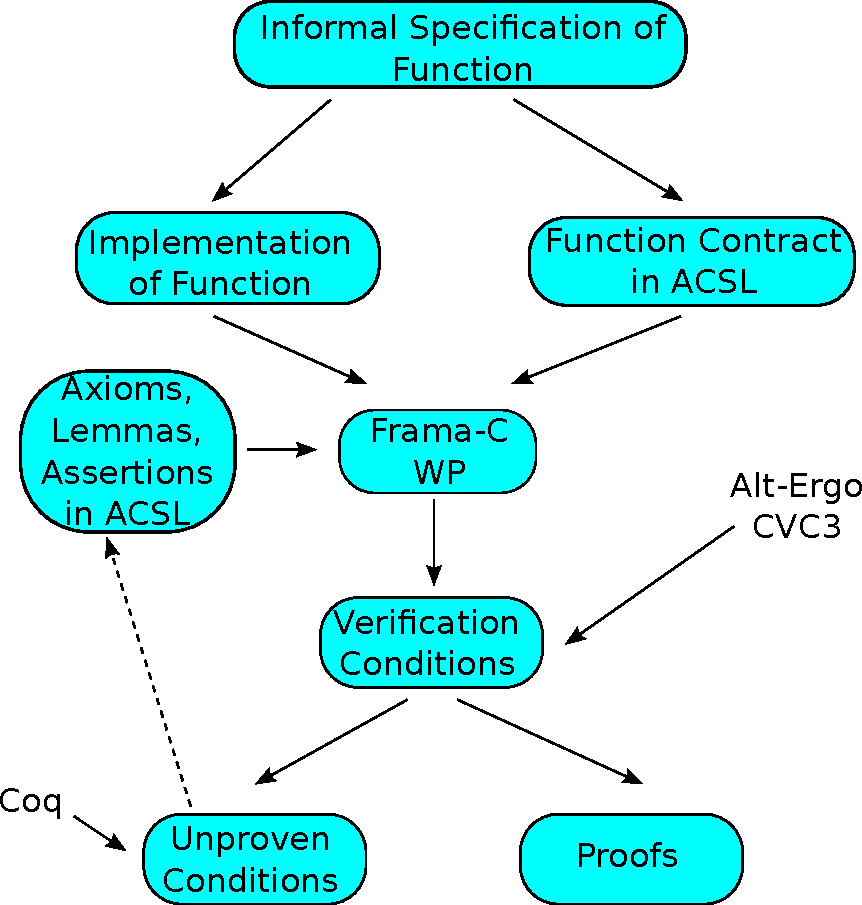
\includegraphics[width=0.50\textwidth]{figures/method-bitwalker.pdf}
\caption{\label{fig:method} The method to formally verify the Bitwalker.}
\end{figure}

Starting point is an informal specification of a function with which in mind
a implementation is written and on which basis the formal specification is created.
The formal specification of a function is a so-called function contract
which contains preconditions to express what a function expects from its caller
and postconditions to state the guarantees after the execution.
The specification language is called 
\acsl (ANSI\slash ISO-\isoc Specification Language)~\cite{acsl} 
which is a formal language to express behavioral properties of \isoc programs.

Moreover, it is the specification language associated with 
the verification platform \framac~\cite{FramaC}
which we use along with its plug-in \wpframac~\cite{wp}.
Within \framac, \wpframac enables the deductive verification of
\isoc programs that have been annotated with \acsl.
\wpframac generates verification conditions which are submitted to external 
automatic or interactive theorem provers.
A function is then verified if each verification condition is discharged
by at least one prover.

Figure~\ref{fig:method} shows that we first apply the automatic
theorem provers \altergo~\cite{alt-ergo} and \cvc~\cite{cvc3}
and then apply the
interactive theorem prover \coq~\cite{Coq}
for the still unproven conditions in order to automate as much as possible.
Moreover, unproven conditions motivate to give some extra information
in the form of axioms, lemmas and assertions in \acsl, 
since they can ease the search of a proof.
One need to be careful with axioms because they can yield contradictions
and thus make the proof system unsound.
This is different for lemmas and assertions
because \wpframac will generate additional verification conditions for them.

In order to prove the absence of run time errors we use
the \inl{rte} option of \wpframac that automatically introduce \acsl
assertions. If all these assertions can be proven, then
the absence of run time errors is guaranteed.


\subsection{The Function \peek}
\label{peek}


In this section we examine the function \peek.
Initially, we provide an informal specification 
followed by an implementation.
We then derive a formal specification on the basis of the informal one. 
Finally, we present the results of the deductive verification with \framac and \wpframac.


\subsubsection{Informal Specification}
\label{informal-peek}


We first introduce some auxiliary concepts and formulate general assumptions:

\begin{itemize}
\item
A \emph{bit stream} is an array containing elements of type \verb"uint8_t".

A bit stream of length $n$ contains $8n$ bits.

\item
A bit stream is \emph{valid} if the array is valid.

\item 
A bit stream can be indexed both by its array indices
and its \emph{bit indices}.

Figure~\ref{fig:bitstream-indices} shows the difference between 
array indices and bit indices in a bit stream.
The two bit indices, 0~and~14,
mark bit positions in the first and second array element, respectively.

\begin{figure}[hbt]
\begin{center}
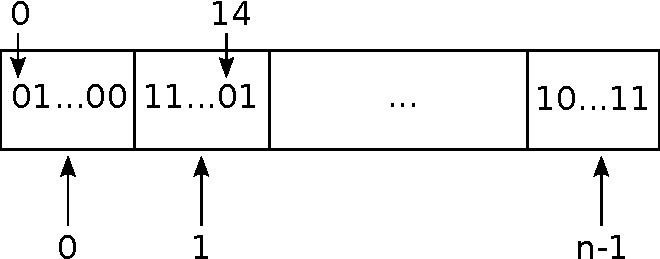
\includegraphics[width=0.40\textwidth]{figures/array_as_stream.pdf}
\caption{\label{fig:bitstream-indices} Array indices and bit indices in a bit stream}
\end{center}
\end{figure}


\item
A \emph{bit sequence} is a consecutive sequence of bits within a bit stream
as represented in Figure~\ref{fig:bitsequence}.
\begin{figure}[hbt]
\begin{center}
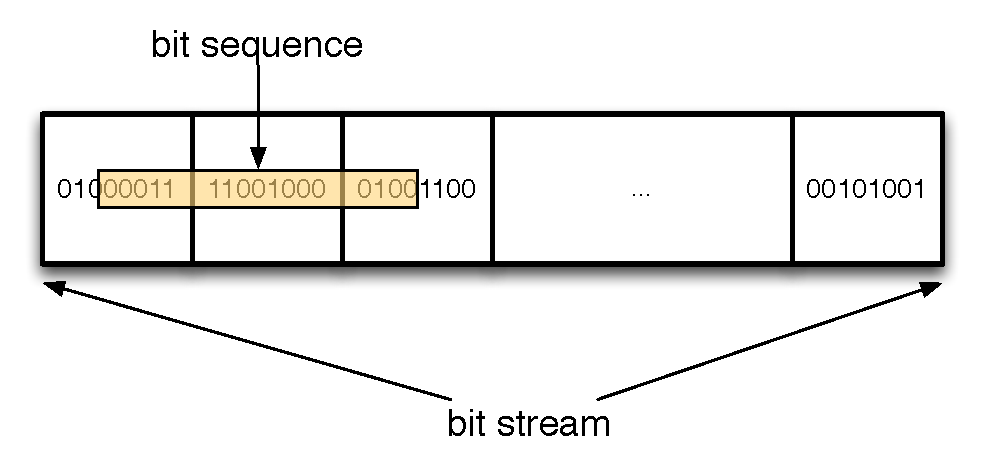
\includegraphics[width=0.40\textwidth]{figures/bit_sequence.pdf}
\caption{\label{fig:bitsequence} A bit sequence within a bit stream}
\end{center}
\end{figure}

A bit sequence is given by the position of its first bit (a bit index in the bit stream)
and its \emph{length}, that is, the number of bits it contains.

\item A bit sequence of length $l$ that starts at bit index $p$ is \emph{valid}
     with respect to a bit stream of length $n$ if the following conditions are
     satisfied
     \begin{align*}
         0 &\leq p \leq 8n \\
         0 &\leq p + l \leq 8n
     \end{align*}

\item 
We assume that the C-types \texttt{unsigned int} and \texttt{int}
have a width of~32~bits.

\end{itemize}

Now we specify \peek with the introduced auxiliary concepts.
The function \texttt{Bitwalker\_Peek} reads a bit sequence from a bit stream
and converts it to an integer.

Its function signature reads as follows:

\begin{lstlisting}[style=acsl-block]
uint64_t  Bitwalker_Peek(unsigned int Startposition, 
                         unsigned int Length,
                         uint8_t Bitstream[],
                         unsigned int BitstreamSizeInBytes);
\end{lstlisting}

The arguments have the following purpose:
\begin{itemize}
    \item \texttt{Startposition} is the bit index in the bit stream 
    where the bit sequence starts.
    \item \texttt{Length} is the length of the bit sequence.
    \item \texttt{Bitstream} is the array which provides the bit stream.
    \item \texttt{BitstreamSizeInBytes} is the length of the array 
    containing the bit stream. 
\end{itemize}


The following preconditions shall hold for the function arguments:
\begin{itemize}
\item \texttt{Bitstream} is a valid array of length \verb"BitstreamSizeInBytes"

\item \texttt{Length} $\leq$ \texttt{64} and

\item \texttt{Startposition + Length} $\leq$ \verb"UINT_MAX".
\end{itemize}

Note that additional constraints are implicitly expressed by the use
of \emph{unsigned} integer types.

We continue with a more precise description of the desired behavior of \peek.
As mentioned, the function \texttt{Bitwalker\_Peek} reads a bit sequence from a bit stream
and converts it to a 64-bit unsigned integer.

The left most bit of the bit sequence is interpreted as
the most significant bit.
Thus, for a bit sequence $(b_0, b_1,\ldots,b_{n - 1})$ the function
returns the sum
\begin{align}
    b_0 \cdot 2^{n - 1} + b_1\cdot 2^{n - 2} + \ldots + b_{n-1}\cdot 2^0
    =
    \sum_{i=0}^{n-1} b_i \cdot 2^{(n - 1) - i} 
\end{align}

If the bit sequence is not valid, then the function returns \texttt{0}.
This increases the robustness of the function.

\subsubsection{Implementation}
\label{impl-peek}
 
Listing~\ref{fig:impl-peek} shows the \isoc implementation of \peek 
for which we aim to verify that it fulfills the informal specification.
The case where the bit sequence is not valid is handled by the \texttt{if}-statement.
For a valid sequence the summation of the bits is done in the \texttt{for}-loop.
The array \texttt{BitwalkerBitMaskTable} is a \texttt{const} helper array 
to select a single bit in the \texttt{Bitstream}.

\begin{listing}[hbt]
\begin{minipage}{\textwidth}
\lstinputlisting[style=acsl-block, frame=single]{./figures/peek.impl}
\end{minipage}
\caption{\label{fig:impl-peek} Implementation of \peek}
\end{listing}

The implementation uses a great amount of bit operations
which is quite a challenge for the formal verification.
We will discuss this further in section~\ref{issues}.

\FloatBarrier
\clearpage

\subsubsection{Formal Specification with \acsl}
\label{formal-peek}

In order to verify that the given implementation of \peek fulfills 
the informal specification, we have to formalize the specification.
Listing~\ref{fig:spec-peek} shows such a formalization in \acsl for \peek.

\begin{listing}[hbt]
\begin{minipage}{\textwidth}
\lstinputlisting[style=acsl-block, frame=single]{./figures/peek.spec}
\end{minipage}
\caption{\label{fig:spec-peek} Formal specification of \peek in \acsl}
\end{listing}

We specify a function contract for \peek containing preconditions
and postconditions introduced by the key words \inl{requires}
and \inl{ensures}, respectively.
In addition, the \acsl language provides the \inl{assigns} clause to specify 
that a function is not allowed to change memory locations other than the ones 
explicitly listed. 
When no \inl{assigns} clauses are specified, 
the function is allowed to modify every visible variable. 

The three preconditions for the function arguments of the informal specification 
are formalized straight forward in the function contract also by three preconditions.
For the first one we use the predicate \inl{IsValidRange}
which we specified in \acsl in order to state that the \inl{Bitstream}
is a valid array of length \inl{BitstreamSizeInBytes}.
Furthermore, we claim that \peek does not alter any memory locations
apart from internal function variables via the \inl{assigns} clause.

Moreover, we use so-called behaviors in \acsl for a distinction of the two cases
from the informal specification.
The cases are discriminated through the predicate \texttt{ValidBitIndex}
which indicates whether a bit sequence is valid or not.
The first behavior \texttt{out\_of\_range} represents the robustness 
case where the bit sequence is not valid and 
the second behavior specifies the expected behavior in the normal case.

In both cases we state what the result of \peek shall be 
as postconditions. In addition, we use a negated form of
a predicate called \inl{TooBig} in the last postcondition of
the normal case. This postcondition was introduced to verify
that the functions \peek and \poke interact correctly.
Therefore, we will discuss this postcondition in section~\ref{interaction}.

Since the implementation of \peek contains a loop,
we need a loop specification containing a variant for the termination
proof and some invariants to enable the automatic theorem provers
to verify the postconditions.
Although this loop specification is important for the verification,
it is not in the sense to formalize the informal specification.

Since we verify the implementation in respect to the formal specification, 
it is crucial that it matches the informal one. 
Therefore, we reviewed the accordance of both specifications.

\FloatBarrier

\subsubsection{Formal Verification with \framac/\wpframac}
\label{verification-peek}

In this section we present the current state of the verification results 
for \peek.
Table~\ref{tab:results-peek} discriminates the results for
three different types of verification conditions (VCs).

\begin{table}[hbt]
  \centering
  \begin{tabular}[htb]{lccc}
    \toprule
     & \# VC & Proven VCs & Verification rate in \%\\
    \midrule
    lemmas & $1$ &$0$ & $0$ \\
    %\midrule
    rte-assertions&$9$&$5$&$55$\\
    rest &$18$ &$17$&$94$\\
 %   \bottomrule
%    &$27$&$22$&$81$\\
    \bottomrule
  \end{tabular}
  \caption{Verification Results of \peek}
  \label{tab:results-peek}
\end{table}


The first row contains the lemmas we used to ease the verification for the automatic theorem provers.
While the second row contains the \inl{rte}-assertions 
concerning the absence of run time errors.
The third row shows all other verification conditions for \peek
which are mainly about for correct functional behavior.
However, they also contain the postconditions for the robustness cases
and the loop specification.

For each row we listed the total number of generated verification conditions,
the number of proven verification conditions and the verification rate
that is the percentage of proven verification conditions. 

The verification rate for the \inl{rte}-assertions are very low 
due to the difficulty for \framac to deal with bit operations.
In order to increase this rate, we will verify the absence
of run time errors separately and will provide additional lemmas and axioms
to ease the verification.
We point out some of the related challenges in section~\ref{issues}.



\FloatBarrier



\subsection{The Function \poke}
\label{poke}


In this section we examine the function \poke
in the same manner as we did it for \peek in section~\ref{peek}.

\subsubsection{Informal Specification}
\label{informal-poke}

The function \poke converts an integer to a bit sequence and writes it
into a bit stream.
Its function signature reads as follows:
\begin{lstlisting}[style = acsl-block]
int      Bitwalker_Poke(unsigned int Startposition,
                        unsigned int Length,
                        uint8_t Bitstream[],
                        unsigned int BitstreamSizeInBytes,
                        uint64_t Value);
\end{lstlisting}


%\subsubsection*{Arguments}
The arguments have the following purpose:

\begin{itemize}
    \item \texttt{Startposition} is the bit index in the bit stream 
    where the bit sequence starts.
    \item \texttt{Length} is the length of the bit sequence.
    \item \texttt{Bitstream} is the array which provides the bit stream.
    \item \texttt{BitstreamSizeInBytes} is the length of the array 
    containing the bit stream. 
    \item \texttt{Value} is the integer which shall be converted into a bit sequence.
\end{itemize}


%\subsubsection*{Preconditions}
The following preconditions shall hold for the function arguments:

\begin{itemize}
\item \texttt{Bitstream} is a valid array of length \verb"BitstreamSizeInBytes"

\item \texttt{Length} $<$ \texttt{unsigned int}.

\item \texttt{Startposition + Length} $\leq$ \verb"UINT_MAX".
\end{itemize}

Note that additional constraints are implicitly expressed by the use
of \emph{unsigned} integer types.


%\subsubsection*{Description}
Now we can specify \poke as follows:
The function \poke converts a 64-bit unsigned integer to a bit sequence and 
writes it into a bit stream.

For $0 \leq x$ exists a shortest sequence of~0 and~1
$(b_0, b_1,\ldots,b_{n - 1})$
such that
\begin{align}
    \sum_{i=0}^{n-1} b_i \cdot 2^{(n - 1) - i} = x.
\end{align}

The function \poke tries to store the sequence $(b_0, b_1,\ldots,b_{n - 1})$
in the bit sequence of \texttt{Length} bits that starts
at bit index \texttt{Startposition}.

The return value of \poke depends on the following three cases:

\begin{itemize}
\item 
If the bit sequence is valid, then there are two cases:

\begin{itemize}
\item
If $\texttt{Length} \geq n$, then  the sequence
$(\overbrace{0,\ldots,0}^{\texttt{Length}-n},b_0, b_1,\ldots,b_{n - 1})$
is stored in the bit stream starting at \texttt{Startposition}.
The return value of \poke is 0.

\item
If $\texttt{Length} < n$, then the
sequence $(b_0, b_1,\ldots,b_{n - 1})$ cannot be stored and\\
\poke returns~$-2$.
\end{itemize}

\item 
If the bit sequence is not valid, then \poke returns~$-1$.
\end{itemize}

\subsubsection{Implementation}
\label{impl-poke}
Listing \ref{fig:impl-poke} shows the implementation of \poke
which discriminates three cases. The first two are the robustness cases
of the informal specification and the last one is
the normal case where the function actually writes into the bit stream.
Similar to \peek a lot of bit operations are used. 

\begin{listing}[hbt]
\begin{minipage}{\textwidth}
\lstinputlisting[style=acsl-block, frame=single]{./figures/poke.impl}
\end{minipage}
\caption{\label{fig:impl-poke} Implementation of \poke}
\end{listing}



\FloatBarrier

\subsubsection{Formal Specification with ACSL}
\label{formal-poke}

Listing~\ref{fig:spec-poke} shows the function contract of \poke.
The case independent preconditions of the informal specification 
are reflected by the  first three \inl{requires}-clauses at the beginning of the contract.
\poke modifies the \inl{Bitstream} and reads the array
\inl{BitwalkerBitMaskTable} thus we need to express 
that the two arrays must have separated memory locations. 
Therefore, we use the predicate \inl{separated} in the fourth \inl{requires}-clause.
Furthermore, in the following \inl{assigns}-clause we specify the memory locations which 
can be altered by the function.

We specify the three cases of \poke by using behaviors. 
The first behavior \inl{out\_of\_range} occurs if the given bit sequence is not valid with respect to the \inl{Bitstream}. 
The second behavior \inl{value\_too\_big} covers the case that the value \inl{Value} 
is not representable with only \inl{Length} bits.

Finally, the behavior \inl{normal} assumes 
that \inl{Value} is not too big and the bit sequence is valid. 
Here, \poke writes the particular bit sequence into \inl{Bitstream} 
while all other memory locations are unaltered.
For all behaviors there is one postcondition to state what
the return value shall be in this case.


\begin{listing}[hbt]
\begin{minipage}{\textwidth}
\lstinputlisting[style=acsl-block, frame=single]{./figures/poke.spec}
\end{minipage}
\caption{\label{fig:spec-poke} Formal Specification of \poke}
\end{listing}



\FloatBarrier

\subsubsection{Formal Verification with Frama-C/WP}
\label{verification-poke}

In this section we present the current state of verification results of 
for \poke.
The results are shown in Table~\ref{tab:results-poke}.
 We listed the different verification conditions 
 row by row like we did it for \peek.

The function \poke has significantly more unproven verification conditions than \peek
this is because it is more complex and alters memory locations via bit operations.
Therefore, we will verify the absence of run time errors separately as well.

\begin{table}[hbt]
  \centering
  \begin{tabular}[h]{lccc}
    \toprule
     & \# VC & Proven VCs & Proven VCs in \%\\
    \midrule
    lemmas & $1$ &$0$ & $0$ \\
    %\midrule
    rte-assertions&$19$&$7$&$36$\\
    rest &$49$ &$38$&$77$\\
    %\bottomrule
    %&$68$&$45$&$66$\\
    \bottomrule
  \end{tabular}
  \caption{Verification Results of \poke}
  \label{tab:results-poke}
\end{table}

\FloatBarrier


\subsection{Interaction of \peek and \poke}
\label{interaction}


In this section we examine the interaction of 
\peek and \poke. The functions shall be inverse to each other
in respect to the normal cases of both functions.
In the following we provide a formal specification and present
our verification results.


\subsubsection{Formal Specification with ACSL and C}

For the specification of the interaction we have two auxiliary \isoc functions:
The first one to call first \poke on a bit stream and then \peek
and the second one to do it the other way around.

Figure~\ref{fig:poke-peek} shows the straight forward implementation 
of the first helper function along with its \acsl contract.
The contract contains a lot of preconditions because we
only specify an interaction for the case that both functions are in their normal
cases. The reader can compare the preconditions with them from
the contracts of \peek and \poke with respect to the \inl{normal} behaviors.
As a postcondition we formulate that \peek reads exactly the value
written by \poke.

\begin{listing}[hbt]
\begin{minipage}{\textwidth}
\lstinputlisting[style=acsl-block, frame=single, linerange=3-20]{./figures/Peek_Poke_inverse.c}
\end{minipage}
\caption{\label{fig:poke-peek} Specification of interaction when first calling \poke.}
\end{listing}

Figure~\ref{fig:peek-poke} shows the straight forward implementation 
of the second auxiliary function along with its \acsl contract.
In contrast to the first function, we work with two bit streams.
With \peek a certain bit sequence is read out from one bit stream
and written via \poke into the other one.
Therefore, we formulate as a postconditions that
the two bit streams are equal in these certain ranges.

\begin{listing}[hbt]
\begin{minipage}{\textwidth}
\lstinputlisting[style=acsl-block, frame=single, linerange=22-43]{./figures/Peek_Poke_inverse.c}
\end{minipage}
\caption{\label{fig:peek-poke} Specification of interaction when first calling \peek.}
\end{listing}

 \FloatBarrier

\subsubsection{Formal Verification with Frama-C/WP}

All postconditions (and the assertion in figure~\ref{fig:peek-poke})
are verified. Therefore, we succeeded to prove that the 
functions \peek and \poke interact correctly
in respect to their specifications.

Moreover, this verification result serves as a validation for the contracts
of \peek and \poke because the verification of the interaction 
depends on these contracts. Since both functions are called,
the caller has to assure that all preconditions hold
and can then rely on the guarantees given by the postconditions.

As a remark, we extended the contract of \peek by one postcondition 
to ease the verification of the interaction.
The postcondition simply states that the read value is always representable 
by \inl{Length} bits which is obviously always the case,
since the value is the sum of \inl{Length} bits.
The postcondition is needed to assure that the preconditions for the normal case
of \poke are fulfilled when first calling \peek and then \poke.

\clearpage

\subsection{Open Issues}
\label{issues}


Previously, we have seen that \wpframac cannot yet deal very well with bit operations
due to the fact that \wpframac's memory models do not provide 
much information about bit operations.
Therefore, the provers have less options to manipulate the proof goal.
This problem is known and \cealist is working on a solution for the next release.

As a work around one could introduce axioms which provide
additional informations about bit operations. 
The problem by using axioms is that one can introduce wrong facts
yielding contradictions which make the whole proof system unsound. 
Thus, it is an approach one should be really careful with.

Moreover, the chosen automatic theorem provers are generally not very
good when it comes to mixing arithmetic and bit operations.
However, there is an automatic theorem prover namely \z
which is stronger with this. 
At the moment \framac does not provide an interface for \z
but this will probably change with future releases. Thus, we can expect
a better automatic verification rate here.

In addition, we can use the interactive theorem prover \coq to verify 
unproven verification conditions.
Herewith, we can search a proof for a verification condition
on our own by using \coq's various support mechanisms.
Nevertheless, \coq has only the informations provided by the memory
model and the user like the other provers.


\section{SQS}

\section{CEA LIST}

\section{Systerel}

\section{Conlusions}

\nocite{*}
%===================================================
%Do NOT change anything below this line

\end{document}
